\documentclass[12pt,a4paper,notitlepage,onecolumn]{article}
\usepackage[T1]{polski}
\usepackage[utf8]{inputenc}
\usepackage[T1]{fontenc}
\usepackage{graphicx}
\author{Krzysztof Pobożan}
\title{Monitoring aplikacji przy pomocy Prometheusa}
\begin{document}
	\maketitle
	\section{Wstęp}
	Ogólnie że potrzeba aplikacji która pozwoli zgrubsza monitorować zachowanie poszczególnych usług/metod
	\section{Czym jest Prometheus?}
	Narzędzie z otwartym kodem do monitorowania i alertowania.
	\subsection{Funkcje Prometheusa}
	Wielowymiarowy model danych.\\
	PQL\\
	każda instancja sobie\\
	dane zbierane w modelu PULL po http - nie tylko dla Javy\\
	wspiera różne usługi DiscoverySerwis oraz statycznie  w konfigu
	\subsection{Składniki Prometheusa}
\begin{itemize}
	\item Główny serwer zbierający dane
	\item Biblioteki klienckie zbierające dane
	\item Baramka push dla krótko żyjących zadań
	\item Alertmanager
	\item Narzędzia wspierające
\end{itemize}
	\subsection{Arhitektutura}
	\begin{figure}
\centering
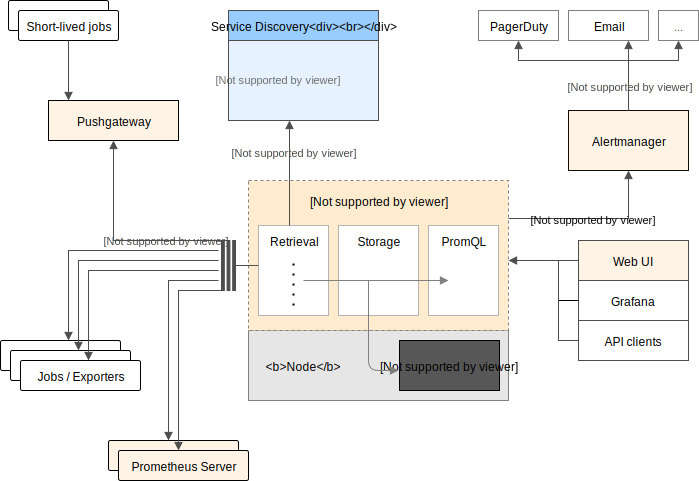
\includegraphics[width=0.7\linewidth]{architecture}
\caption{Architectura prometheusa}
\label{fig:architecture}
\end{figure}

	\section{Rodzaje metryk}
	\section{Agregaty, Alerty i jak tego uzywać}
\end{document}